\documentclass[aspectratio=169]{beamer}
\usepackage[utf8]{inputenc}
\usepackage[T1]{fontenc}
\usepackage[portuguese]{babel}
\usepackage{graphicx}
\usepackage{helvet}



\usepackage{amsmath, amsthm, amsfonts, amscd}
\usepackage{tikz}
\usepackage{tikz-cd}
\usepackage{amssymb}


\renewcommand{\familydefault}{\sfdefault}

\AtBeginDocument{\shorthandoff{"}}

%\usepackage{amsthm}

\newtheorem{proposition}{Proposição}
\newtheorem{theorem}{Teorema}
\newtheorem{corolary}{Corolário}[theorem]
\newtheorem{lemma}{Lema}

\theoremstyle{definition}
\newtheorem{definition}{Definição}

\theoremstyle{remark}
\newtheorem*{example*}{Exemplos}
%\usetheme{Jacquenetta}

%\usetheme{metropolis}
%\metroset{sectionpage=none}

\usetheme[mode=light]{sthlmnord}

%\setbeamertemplate{navigation symbols}{}
%\setbeamercolor{background canvas}{bg=white}
%\setbeamercolor{title}{fg=black}
%\setbeamercolor{frametitle}{fg=black}
%\setbeamerfont{frametitle}{size=\Large, series=\bfseries}

\setbeamertemplate{title page}{
	\vfill
	\begin{centering}
		{\usebeamerfont{title}\usebeamercolor[fg]{title}\Huge \textbf{\inserttitle}}\par
		\vspace{1cm}
		{\usebeamerfont{author}\large \insertauthor}\par
	\end{centering}
	\vfill
	\begin{center}
		
\includegraphics[height=1.6cm]{../figures/logo_unespar.png} \hfill
		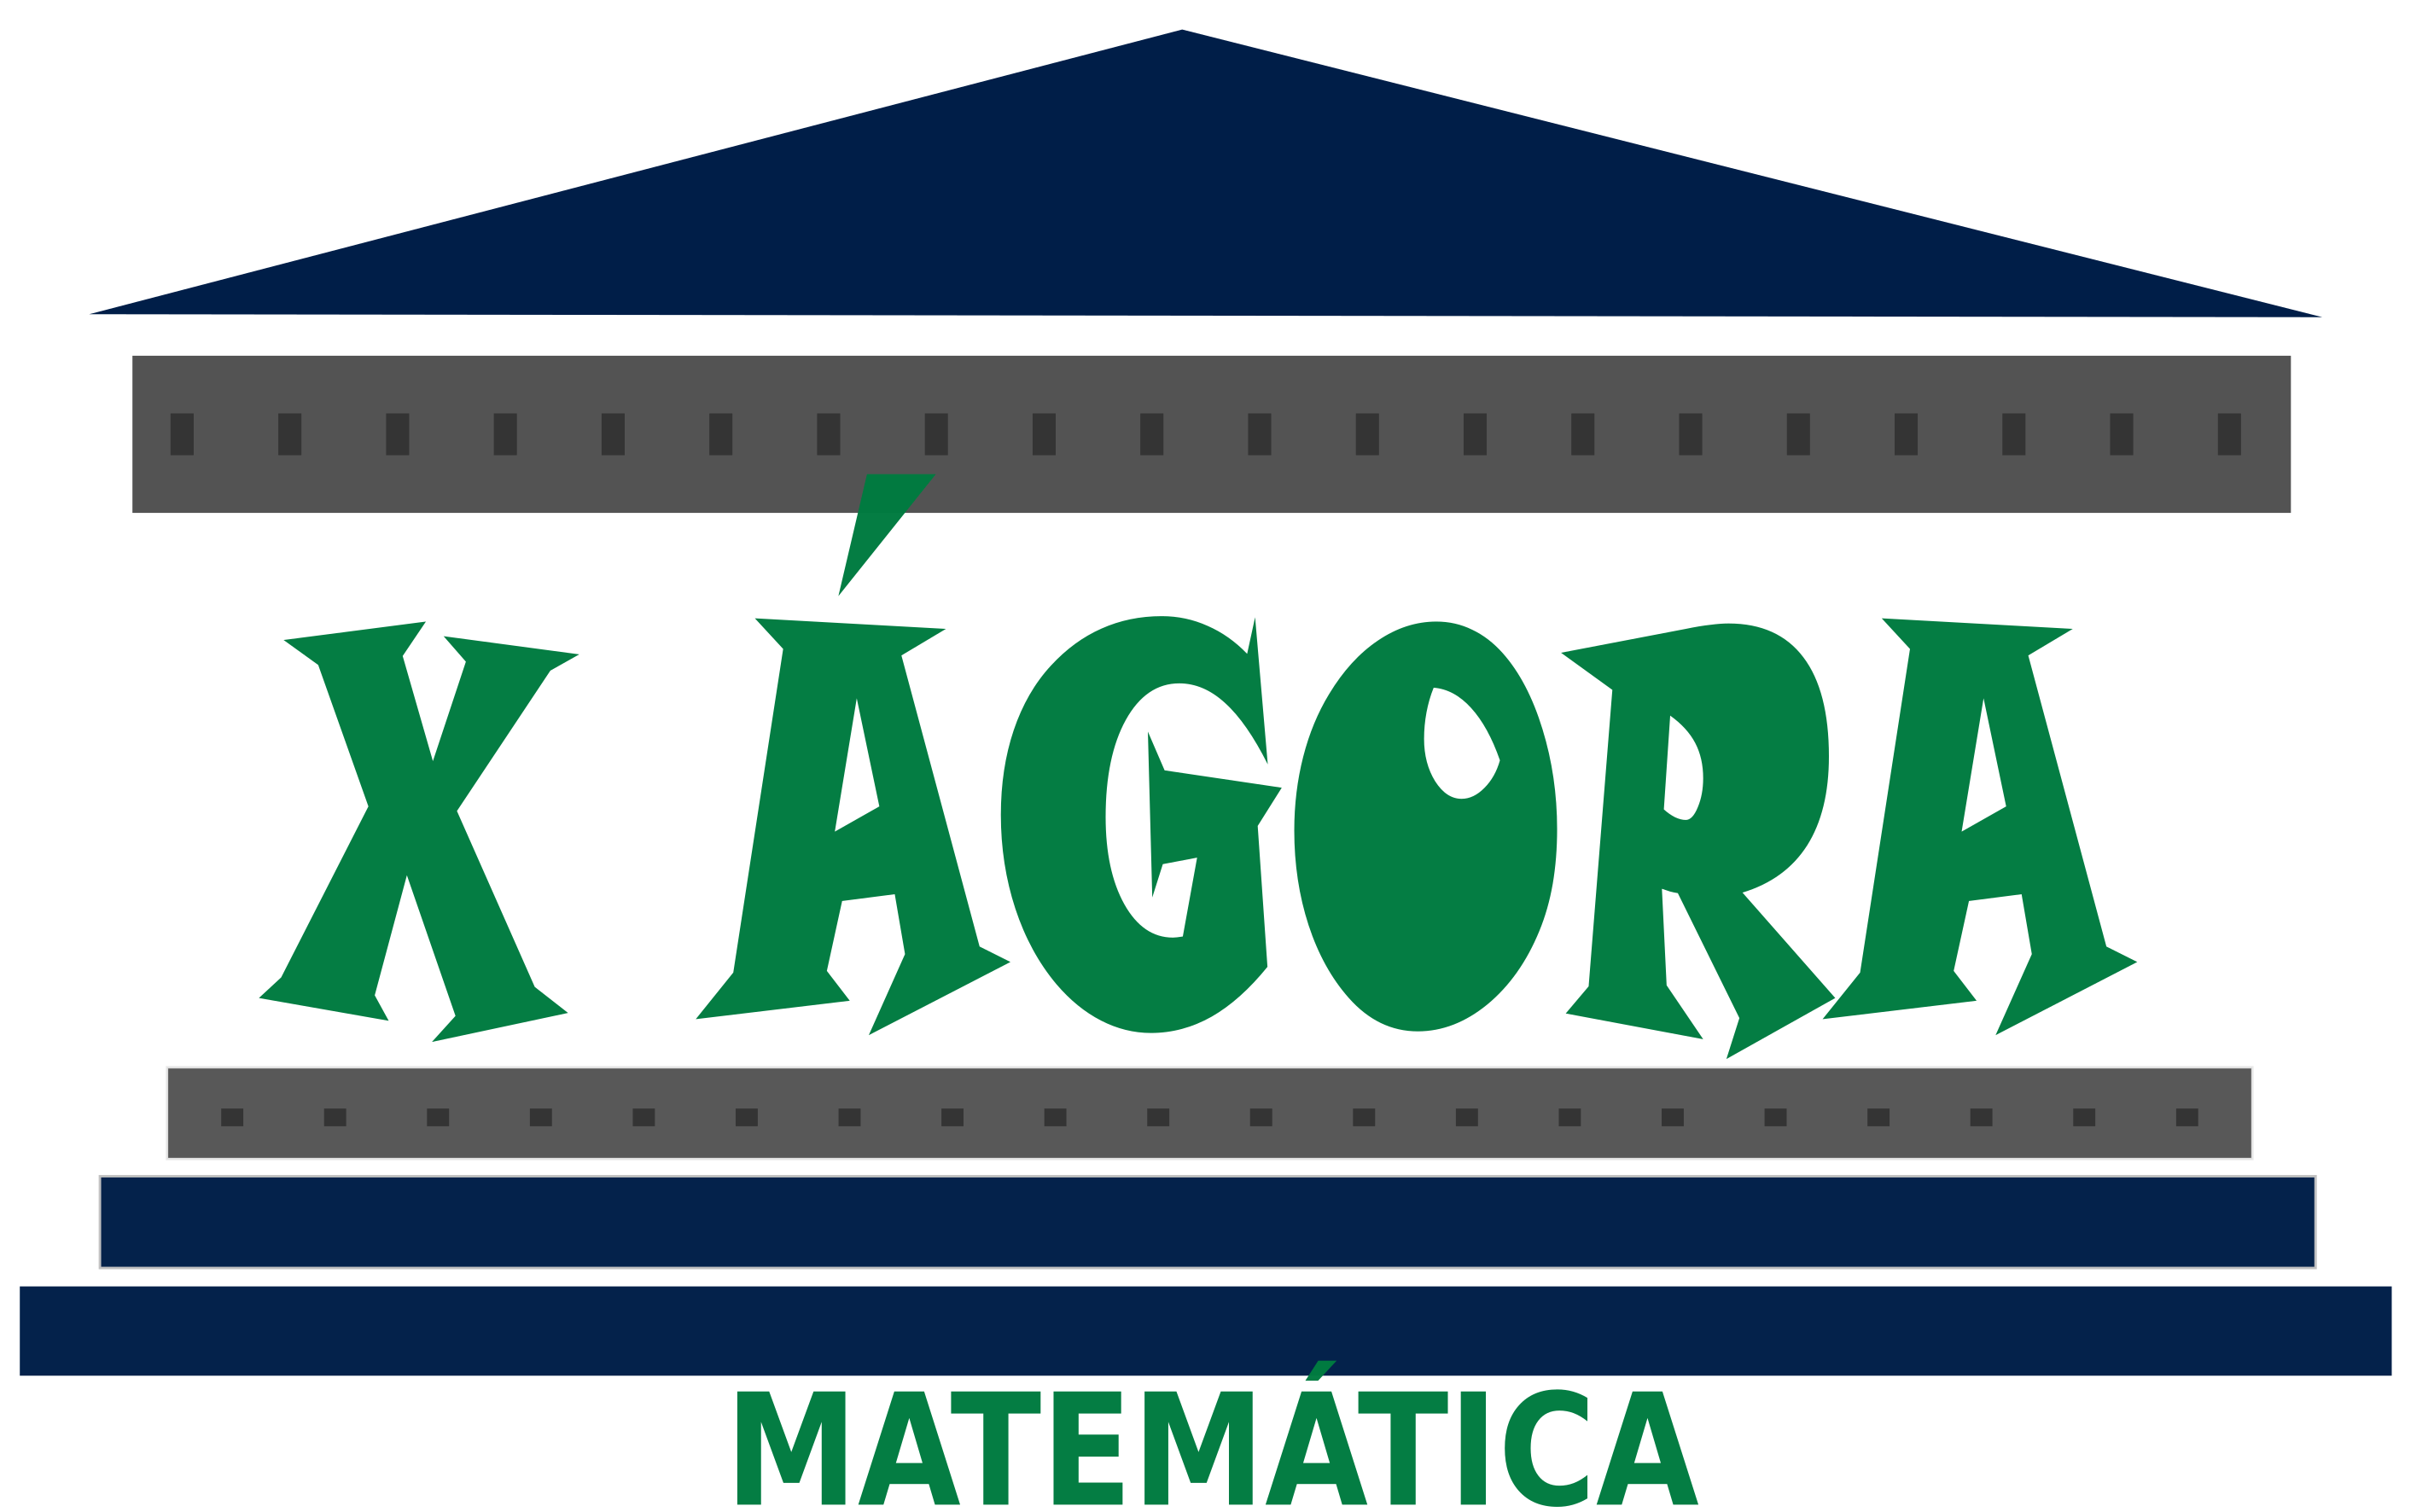
\includegraphics[height=1.2cm]{../figures/logo_evento.png} \hfill
		
\includegraphics[height=1.2cm]{../figures/mat.png} \hfill
		
\includegraphics[height=1.2cm]{../figures/prpgem.png}
	\end{center}
	\vspace{0.2cm}
}

\setbeamertemplate{footline}{
	\ifnum\insertframenumber>1
	\hbox{%
		\begin{beamercolorbox}[wd=.8\paperwidth,ht=1cm,dp=0.5cm,leftskip=1cm]{}
			\scriptsize\color{gray} X Ágora Matemática – Unespar, campus de Campo Mourão
		\end{beamercolorbox}%
		\begin{beamercolorbox}[wd=.2\paperwidth,ht=1cm,dp=0.5cm,right,rightskip=0.8cm]{}
			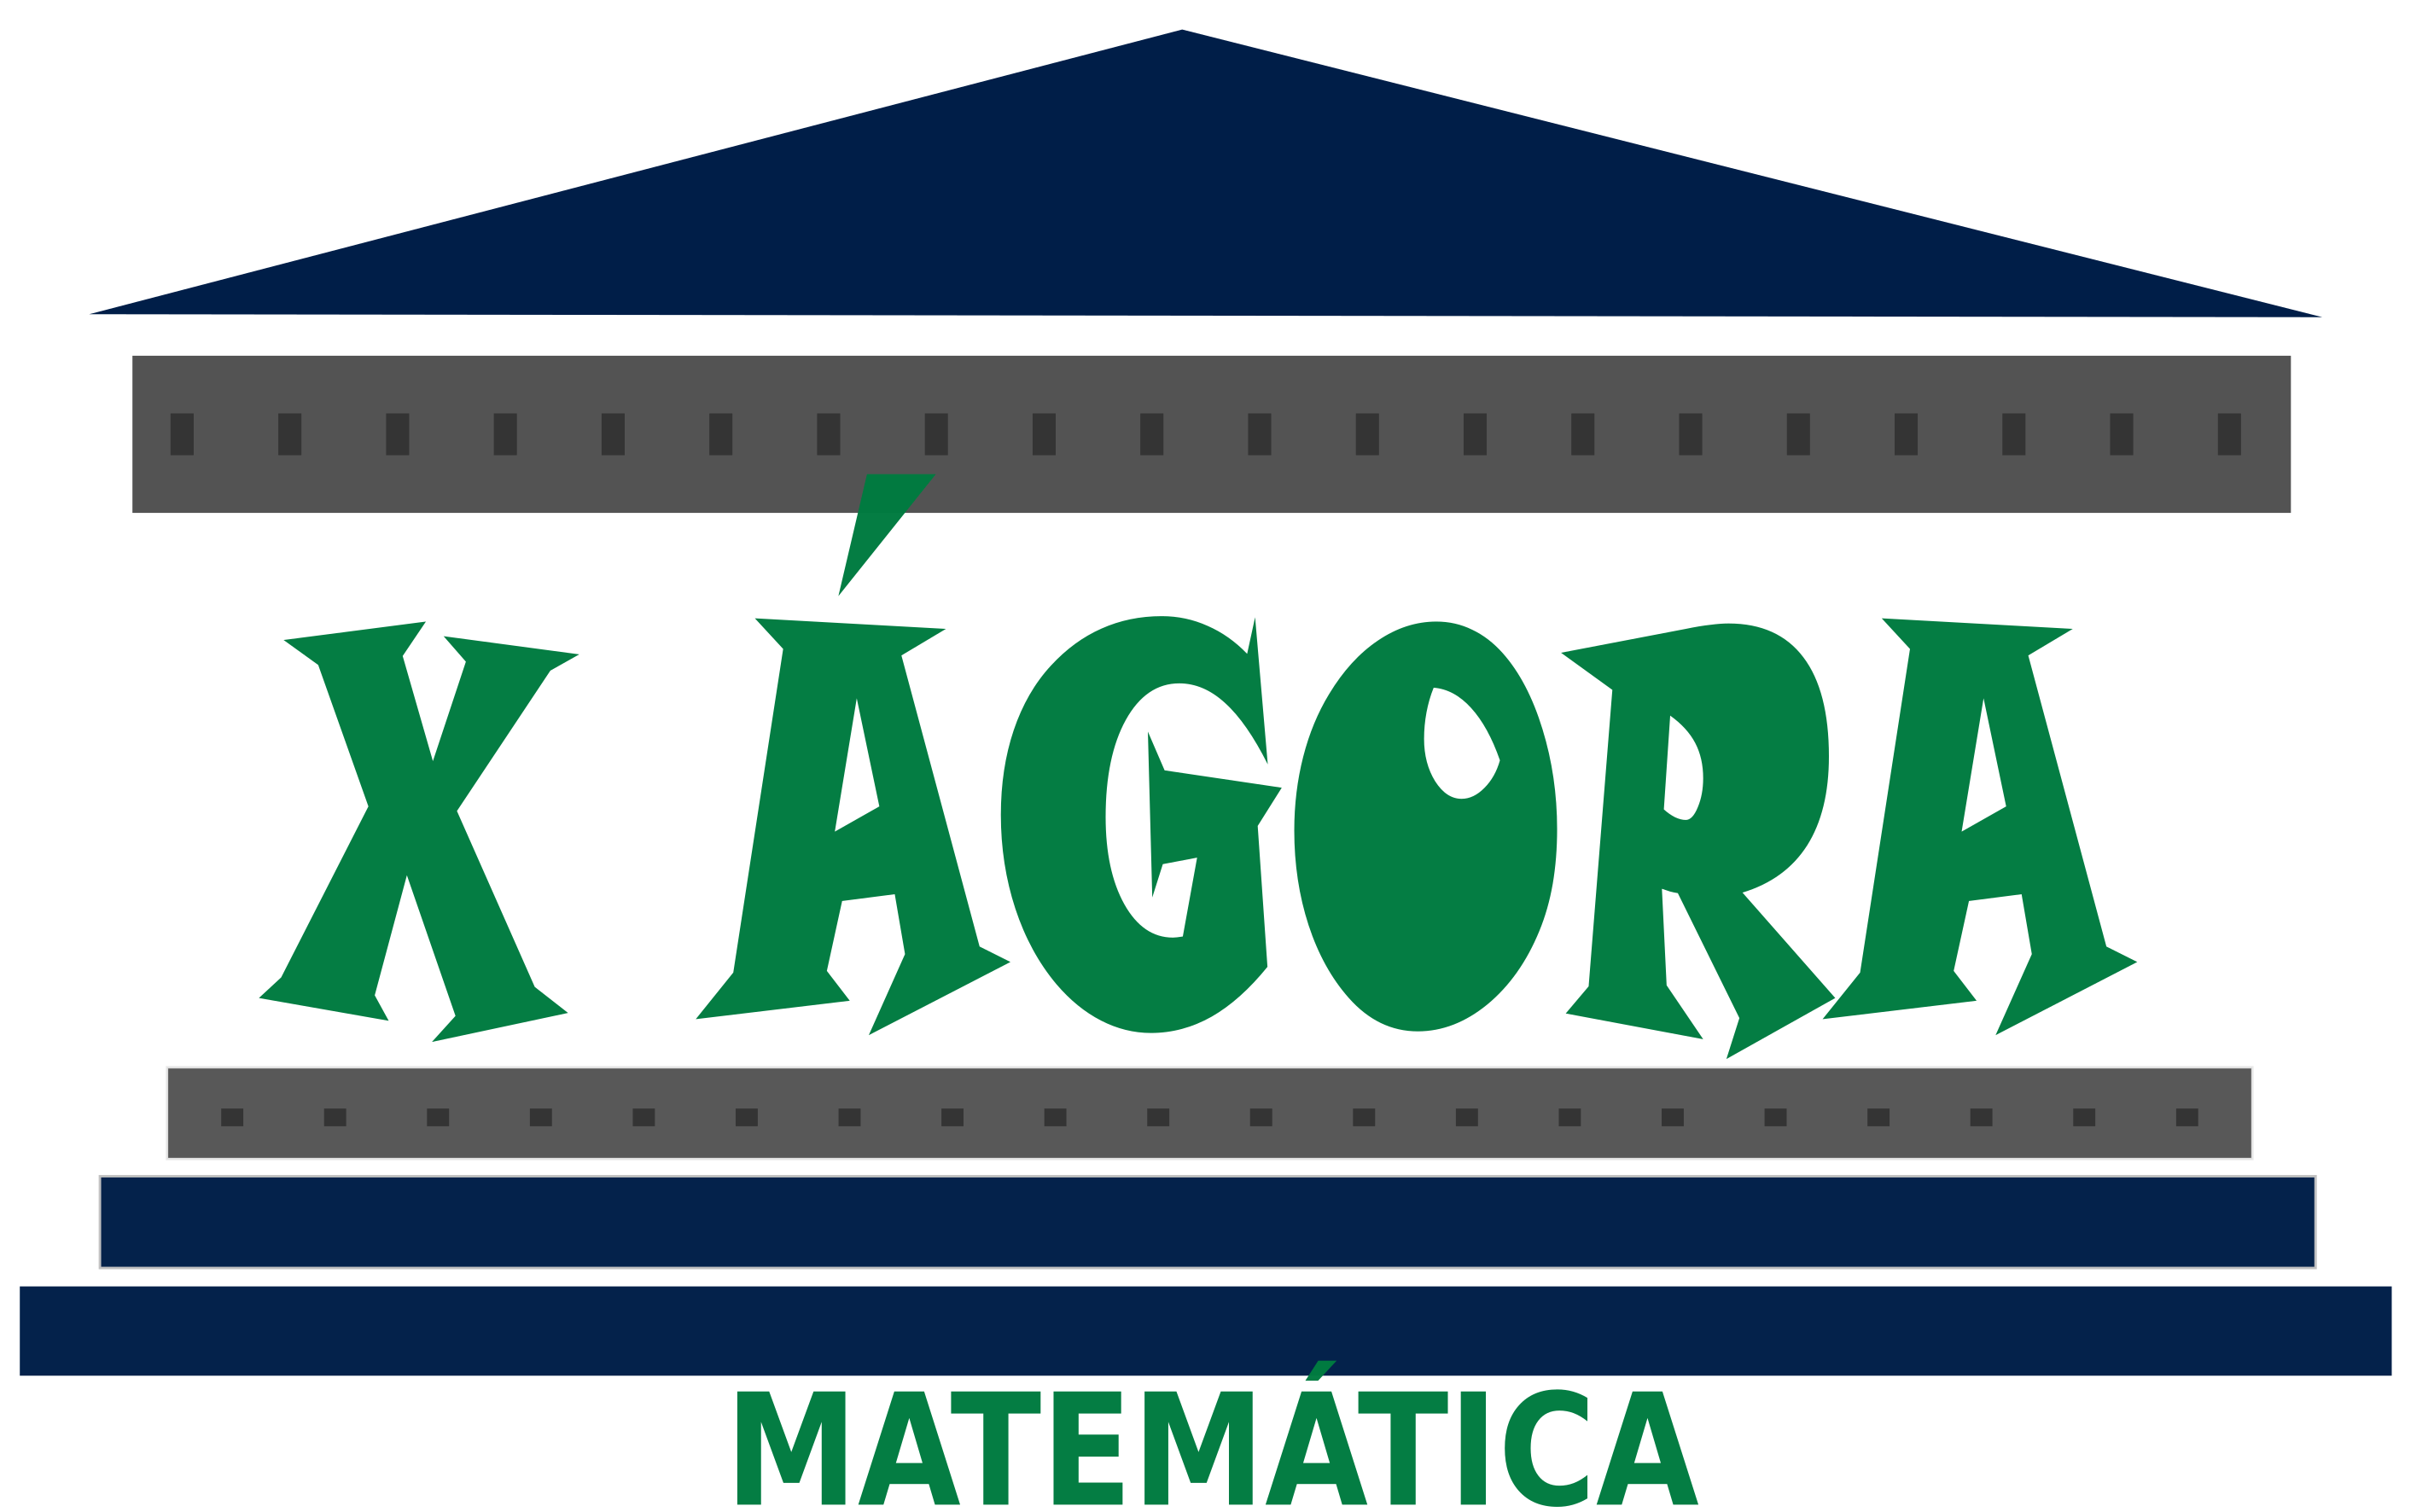
\includegraphics[height=1.2cm]{../figures/logo_evento.png}
		\end{beamercolorbox}%
	}
	\fi
}

%Página de título
\title{Teorema da Base de Hilbert}
\author{\Large
	João Paulo Chiari de Gasperi\\
	Welinton Anderson Rocha\\
	Gislaine Aparecida Periçaro\\
}
\date{}


\begin{document}

% Capa
\begin{frame}[plain]
	\titlepage
\end{frame}

\begin{frame}{Conteúdo}
	\tableofcontents
\end{frame}

% \section{Preliminares}

% \begin{frame}{Relação de Ordem}
% 	\begin{block}{Definição}
% 		Um conjunto $A$ munido com uma relação de ordem parcial, isto é, uma relação anti-simétrica, transitiva e reflexiva é dito um conjunto parcialmente ordenado.
% 	\end{block}
% \end{frame}

% \begin{frame}{Relação de Ordem}
% 	\begin{block}{Proposição}
% 		Se $\Sigma$ é um conjunto parcialmente ordenado, então as seguintes afirmações são equivalentes:
% 		\begin{enumerate}
% 			\item Toda sequência não decrescente $x_{1}\leq x_{2}\leq\dots\leq x_{i}\leq\dots \in \Sigma$  é estacionária, isto é, existe $n>0$ tal que $x_{n}=x_{n+i}, \forall i\geq0$;
% 			\item Todo subconjunto não vazio de $\Sigma$ possui um elemento maximal.
% 		\end{enumerate}
% 	\end{block}
% \end{frame}

% \begin{frame}{Anél}
% 	Um conjunto $A$ munido de duas operações $+$ e $\cdot$ é dito um anel se:
% 	\begin{enumerate}
% 		\pause
% 		\item $A$ é um grupo abeliano sob $+$, isto é, ($A, +$) tem um elemento neutro, todo elemento tem um oposto e $+$ é comutativa e associativa;
% 		      \pause
% 		\item A multiplicação é associativa e é distributiva sobre a adição.
% 	\end{enumerate}

% 	\begin{alertblock}{Anéis comutativos com unidade}
% 		Considerarmos que todo anel é comutativo e possui unidade, isto é, elemento neutro da multiplicação.
% 	\end{alertblock}
% \end{frame}

\section{Módulos}

\begin{frame}{Módulos}
	\begin{block}{Definição}
		Seja $A$ um anel comutativo e com unidade.
		Um $A-$módulo é um grupo abeliano $M$ no qual $A$ age linearmente.
		Isto é, um $A$-módulo é um par $(M, \mu)$, em que $M$ é um grupo abeliano e $\mu:A \times M \to M$ é uma função que satisfaz as seguintes propriedades, indicando $\mu(a, x) = ax$:
		\begin{enumerate}
			\item $a(x+y) = ax + ay$;
			\item $(a+b)x = ax + bx$;
			\item $(ab)x = a(bx)$;
			\item $1x = x$.
		\end{enumerate}
	\end{block}
\end{frame}

\begin{frame}{Exemplos}
	\begin{block}{Ideais}
		Um ideal $\mathfrak{a}\subseteq A$ é um $A$-módulo. Basta definir $\mu(a,x) = ax$ (produto do anel). Em particular, o anel $A$ é um $A$-módulo. A recíproca também é verdade, isto é, todo submódulo de $A$ é um ideal de $A$.
	\end{block}
	\begin{block}{Espaços vetoriais}
		Se $A=k$ é um corpo, então os $A$-módulos são precisamente os $k$-espaços vetoriais.
	\end{block}
\end{frame}

% \begin{frame}{Homomorfismos}
% 	\begin{block}{Definição}
% 		Se $M, N$ são $A$-módulos, então $f:M \to N$ é dito um homomorfismo de $A$-módulos se:
% 		\begin{itemize}
% 			\item $f(x+y) = f(x) + f(y), \forall x,y \in M$ ($f$ é um homomorfismo de grupos entre $M$ e $N$);
% 			\item $f(ax) = af(x), \forall a \in A, x \in M$.
% 		\end{itemize}
% 	\end{block}
% \end{frame}

\begin{frame}{Módulos Noetherianos e Artinianos}
	\begin{block}{Definição}
		\begin{itemize}
			\item Um módulo Noetheriano é tal que toda sequência ascendente de ideais $$M_0 \subseteq M_1 \subseteq \ldots \subseteq M_n$$ é estacionária.
			      \pause
			\item Um módulo Noetheriano é tal que toda sequência descendente de ideais $$M_0 \supseteq M_1 \supseteq \ldots \supseteq M_n$$ é estacionária.
		\end{itemize}
	\end{block}
\end{frame}

\begin{frame}{Exemplo}
	\begin{block}{Espaço Vetorial}
		Um $K-$espaço vetorial, de dimensão finita $n$ é um $K-$módulo Noetheriano e Artiniano.
	\end{block}
	\pause
	\begin{block}{Inteiros}
		$\mathbb{Z}$ como $\mathbb{Z}$-módulo satisfaz a.c.c., mas não d.c.c..

		Como $\mathbb{Z}$ é um domínio principal, um ideal $M$ de $\mathbb{Z}$ é da forma $M=(n)$, para algum $n \in \mathbb{Z}$ com $n \geq 0$. Se $n$ for primo, $(n)$ é maximal, logo não está contido em nenhum outro submódulo de $\mathbb{Z}$. Do contrário, $n=p_{1}p_{2}\dots p_{k}$, com $p_i$ primo para $i=1, \ldots, k$, implicando que $(n)\subseteq(p_{1}\dots p_{k-1})\subseteq(p_{1}\dots p_{k-2})\subseteq\dots \subseteq(p_{1})$, o qual é maximal. Logo, é impossível fazer uma cadeia ascendente infinita de submódulos de $\mathbb{Z}$.
		Para mostrar que $\mathbb{Z}$ não satisfaz d.c.c., tome $\alpha=2 \in \mathbb{Z}$ e considere a sequência $(\alpha)\supset(\alpha^{2})\supset\dots \supset(\alpha^{n})\supset\dots$, a qual é estritamente crescente. Isto mostra que existem módulos Noetherianos que não são Artinianos.
	\end{block}
\end{frame}

\begin{frame}{Anél Noetheriano e Artiniano}
	\begin{block}{Definição}
		Um anel $A$ é dito Noetheriano (respectivamente Artiniano) se for Noetheriano (respectivamente Artiniano) quando considerado como um $A$-módulo, ou seja, se seus ideais satisfazem a.c.c. (respectivamente d.c.c.).
	\end{block}
\end{frame}

\begin{frame}{Equivalência de Noetherianos}
	\begin{block}{Definição}
		$M$ é dito finitamente gerado como um $A$-módulo se existem $m_1, \ldots, m_n \in M$ tais que para todo $x \in M$ podemos escrever $x=\sum_{i=1}^{n}a_im_i$, com $a_i \in A$.
	\end{block}

	\begin{block}{Teorema}
		$M$ é Noetheriano se, e somente se, todo submódulo de $M$ é finitamente gerado.
	\end{block}
\end{frame}

\begin{frame}{Sequências}
	\begin{block}{Definição}
		Uma sequência é uma família $\{ M_{i} \}$ de $A$-módulos e homomorfismos $f_{i}:M_{i-1}\to M_{i}$. Escrevemos
		\[
			\begin{tikzcd}[ampersand replacement=\&]
				\cdots \arrow[r] \& M_{i-1} \arrow[r, "{f_{i}}"] \& M_{i} \arrow[r, "{f_{i+1}}"] \& M_{i+1} \arrow[r] \& \cdots
			\end{tikzcd}
		\]
	\end{block}
	\pause
	\begin{alertblock}{Sequências Exatas}
		Uma sequência é exata em $M_{i}$ se $\mathrm{Im}(f_{i})=\ker(f_{i+1})$. Uma sequência é exata se for exata em todo elemento.
	\end{alertblock}
\end{frame}

\section{Teorema da Base de Hilbert}

\begin{frame}{Lemas}
	\begin{block}{Lema 1}
		Seja
		\[
			\begin{tikzcd}[ampersand replacement=\&]
				0 \ar[r] \& M' \ar[r, "{\alpha}"] \& M \ar[r, "{\beta}"] \& M'' \ar[r] \& 0
			\end{tikzcd}
		\]
		uma sequência exata de $A$-módulos. Então:
		\begin{enumerate}
			\item $M$ é Noetheriano se, e somente se, $M'$ e $M''$ são Noetherianos;
			\item $M$ é Artiniano se, e somente se, $M'$ e $M''$ são Artinianos.
		\end{enumerate}
	\end{block}
\end{frame}

\begin{frame}{Lemas}
	\begin{block}{Lema 2}
		Se $M_{i} (1\leq i\leq n)$ são módulos Noetherianos (respectivamente Artinianos), então $\bigoplus_{i=1}^{n}M_{i}$ é Noetheriano (respectivamente Artiniano).
	\end{block}

	\pause

	\begin{block}{Lema 3}
		$M$ é finitamente gerado se, e somente se, $M$ é isomorfo a um quociente de $A^{n}$ para algum $n>0$.
	\end{block}

	\pause

	\begin{block}{Lema 4}
		Seja $A$ um anel Noetheriano (respectivamente Artiniano). Se $M$ é um $A$-módulo finitamente gerado, então $M$ é Noetheriano (respectivamente Artiniano).
	\end{block}


\end{frame}


\begin{frame}{Teorema da Base de Hilbert}
	\begin{block}{Teorema}
		Se $A$ é um anel Noetheriano, então o anel de polinômios $A[x]$ é Noetheriano.
	\end{block}
\end{frame}

\begin{frame}{Demonstração: Teorema da Base de Hilbert (1/3)}
	\begin{block}{Passo 1: O Ideal dos Coeficientes Principais}
		Seja $\mathfrak{a} \subseteq A[x]$ um ideal. Queremos mostrar que $\mathfrak{a}$ é finitamente gerado.

		\pause
		\vspace{0.3cm}
		Definimos $I$ como o conjunto de todos os \textbf{coeficientes principais} dos polinômios em $\mathfrak{a}$ (acrescido do $0$).

		\pause
		\vspace{0.3cm}
		\begin{itemize}
			\item É possível mostrar que $I$ é um ideal do anel $A$.
			\item Como $A$ é Noetheriano, $I$ é finitamente gerado:
			      $$I = (a_1, a_2, \dots, a_n)$$
		\end{itemize}
	\end{block}
\end{frame}

\begin{frame}{Demonstração: Teorema da Base de Hilbert (2/3)}
	\begin{block}{Passo 2: Redução de Grau}
		Para cada gerador $a_i \in I$, existe um polinômio $f_i \in \mathfrak{a}$ com coeficiente líder $a_i$ e grau $r_i$.
		\begin{itemize}
			\item Seja $r = \max\{r_1, \dots, r_n\}$.
			\item Seja $\mathfrak{a}' = (f_1, \dots, f_n)$ o ideal gerado por eles em $A[x]$.
		\end{itemize}

		\pause
		\vspace{0.3cm}
		Dado qualquer $f \in \mathfrak{a}$ com grau $m \geq r$, podemos \textbf{eliminar seu termo principal} subtraindo uma combinação $h = \sum u_i x^{m-r_i} f_i \in \mathfrak{a}'$.

		\pause
		\vspace{0.3cm}
		O grau de $f - h$ é estritamente menor que o de $f$. Repetindo o processo, reduzimos o grau até que reste um polinômio $g$ com \textbf{grau menor que $r$}.
	\end{block}
\end{frame}

\begin{frame}{Demonstração: Teorema da Base de Hilbert (3/3)}
	\begin{block}{Passo 3: Conclusão usando Módulos}
		Acabamos de mostrar que qualquer $f \in \mathfrak{a}$ pode ser escrito como:
		$$ f = h + g $$
		onde $h \in \mathfrak{a}'$ e $g \in \mathfrak{a}$ é um polinômio de grau $< r$.

		\pause
		\vspace{0.3cm}
		\begin{itemize}
			\item Polinômios de grau $< r$ pertencem ao $A$-módulo $M = \langle 1, x, \dots, x^{r-1} \rangle$.
			\item Logo, $\mathfrak{a} = \mathfrak{a}' + (\mathfrak{a} \cap M)$.
			      \pause
			\item Como $M$ é finitamente gerado sobre $A$ (que é Noetheriano), o submódulo $\mathfrak{a} \cap M$ também é finitamente gerado.
		\end{itemize}

		\pause
		\vspace{0.3cm}
		Portanto, $\mathfrak{a}$ é gerado finitamente pelos $f_i$ unidos aos geradores de $\mathfrak{a} \cap M$.
	\end{block}
\end{frame}

\end{document}